\newpage
\section{Appendix}
\subsection{Tabular Integration by Parts}
\label{appendix:parts}
    One can use a table to perform repeated integration by parts quickly. Suppose we would like to use integration by parts to change the integral of \(u(x)v(x)\) into boundary terms plus the integral of \(u^{(n)}(x)v_{(n)}(x)\). We create a table with alternating signs in the first column, beginning with positive. In the second column, we write \(u(x)\) and its derivatives beneath it while alternating the sign. In the third column, we write \(v(x)\) and its anti-derivatives beneath it. At the end of this process, the table should look as follows.
    \begin{table}[H]
        \centering
        \begin{tabular}{c|rl}
            \(+\) & \(u(x)\) & \(v(x)\)\\
            \hline
            \(-\) &\(u^{(1)}(x)\) & \(v_{(1)}(x)\)\\
            \(+\) & \(u^{(2)}(x)\) & \(v_{(2)}(x)\)\\
            \(-\) & \(u^{(3)}(x)\) & \(v_{(3)}(x)\)\\
            \(\vdots\) &\(\vdots\) & \(\vdots \)\\
            \((-1)^{n-1}\) & \(u^{(n-1)}(x)\) & \(v_{(n-1)}(x)\)\\
            \((-1)^n\) & \(u^{(n)}(x)\) & \(v_{(n)}(x)\)
        \end{tabular}
    \end{table}
    Next, we take the \(i^{\mathrm{th}}\) sign in the left column to be the sign of \(u^{(i)}\), multiply diagonal terms, and add each product.
    \begin{figure}[H]
        \centering
        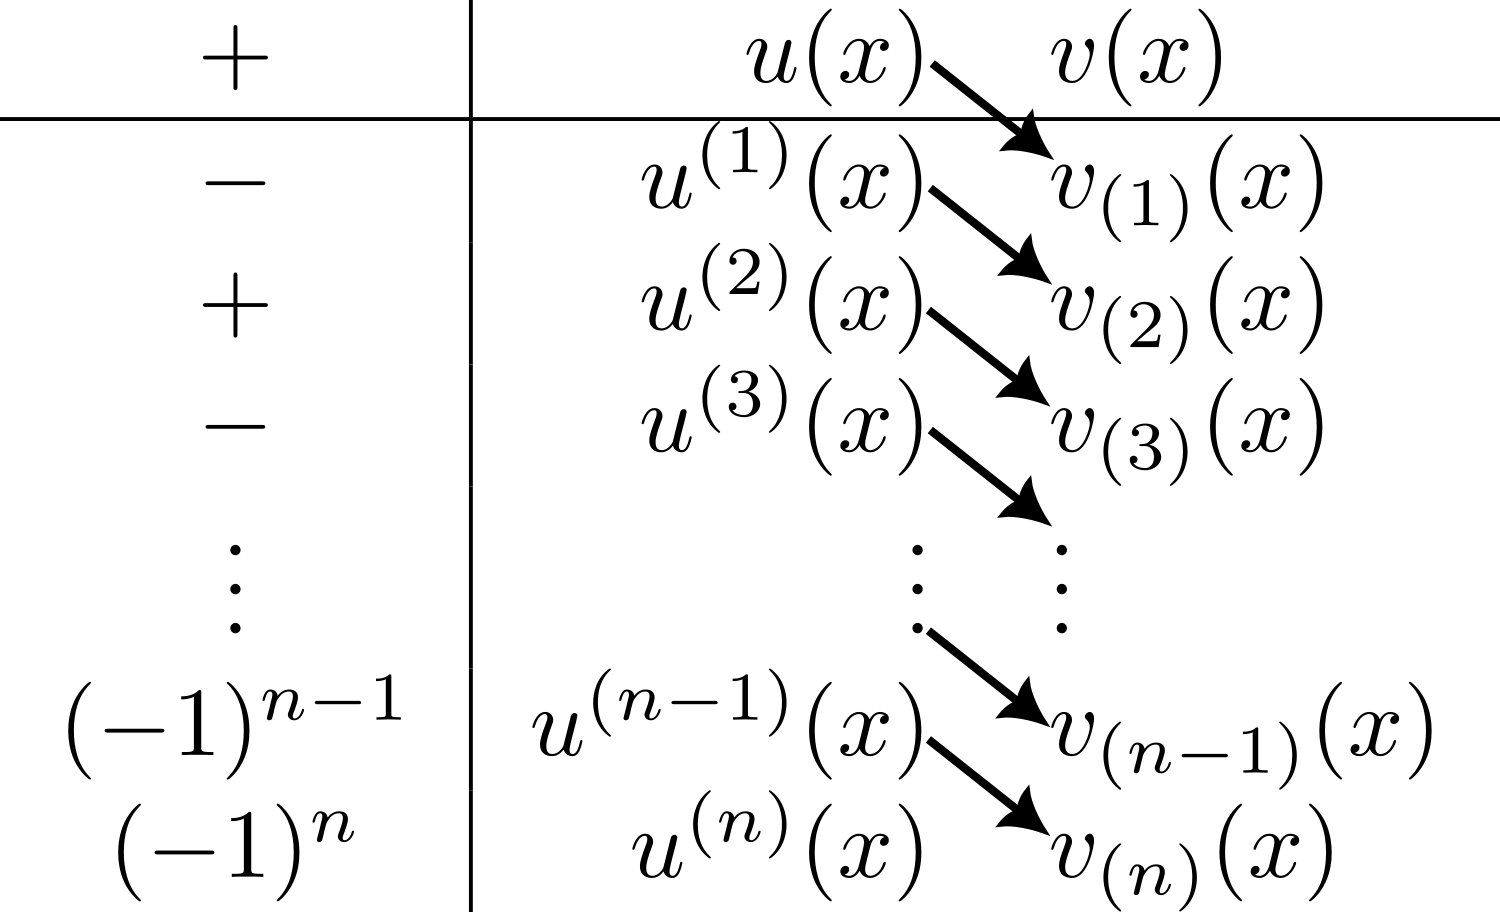
\includegraphics[width=0.34\linewidth]{include/tabular-boundary.png}
    \end{figure}
    These are the boundary terms. Lastly, we multiply the bottom terms together, which becomes the integrand. 
    \begin{figure}[H]
        \centering
        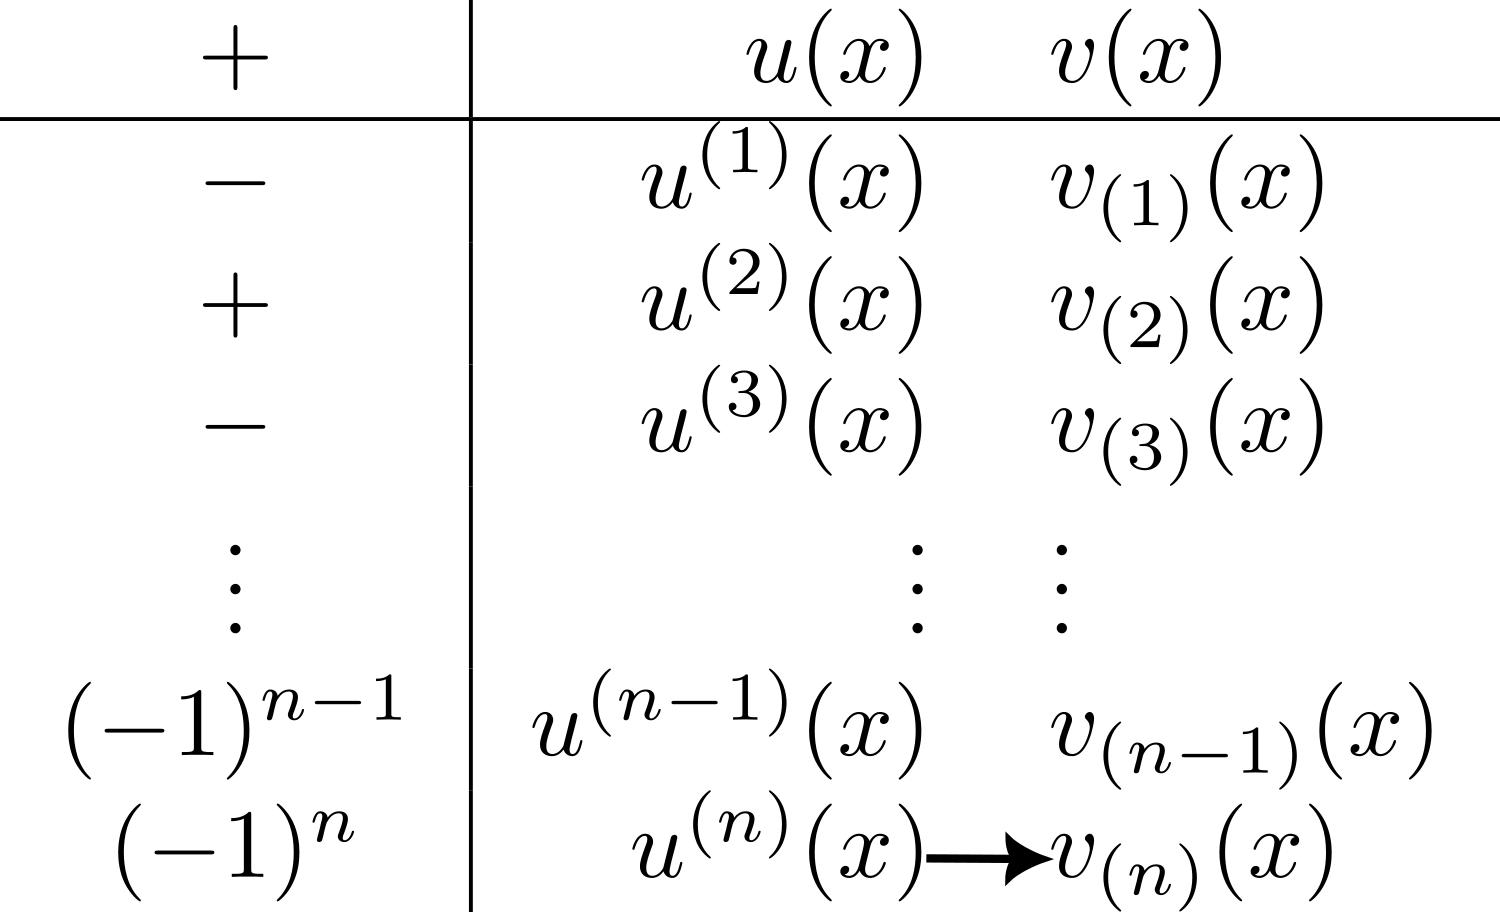
\includegraphics[width=0.34\linewidth]{include/tabular-integrand.png}
    \end{figure}At the end of this process, the original integral has become 
    % \begin{equation*}
    %     \begin{split}
    %         \intl u(x)v(x) dx &= (u(x)v_{(1)}(x)-u^{(1)}(x)v_{(2)}(x)+u^{(2)}(x)v_{(3)}(x) + \cdots + (-1)^{n-1} u^{(n-1)}(x))\biggr\rvert_\mathrm{a}^\mathrm{b}\\ &+ \intl v^{(4)}(x)u(x) dx.
    %     \end{split}
    % \end{equation*}
    \begin{equation*}
        \begin{split}
            \intl u(x)v(x) dx &= \left(\sum_{i=1}^{n} (-1)^{i-1}u^{(i-1)}(x)v_{(i)}(x)\right)\biggr\rvert_\mathrm{a}^\mathrm{b} + \intl u^{(n)}(x)v_{(n)}(x) dx.
        \end{split}
    \end{equation*}
\subsection{The Mean Value Theorem}
    The mean value theorem states that for all \(f:[\lima,\limb]\to \mathbb{R}\) such that \(f\) is continuous on \([\lima,\limb]\), and differentiable on \((\lima, \limb)\), then 
    \begin{equation*}
        \exists c \in (\lima, \limb) : f'(\text{c}) = \frac{f(\limb)-f(\lima)}{\limb-\lima}
    \end{equation*}
    and thus,
    \begin{equation*}
        f'(c)(\limb-\lima) = f(\limb)-f(\lima)
    \end{equation*}
    By integrating \(f'(x)\) , we see that
    \begin{equation*}
        \begin{split}
            \int_\lima^\limb f'(x) dx &= f(\limb)-f(\lima)\\
            &=f'(\text{c})(\limb-\lima)
        \end{split}
    \end{equation*}
\subsection{Big O Notation} \label{sec:BigO}
Big O notation is used to describe the limiting behavior of a function as the argument tends to some value or infinity. By \(f(x)=O(g(x))\) as \(x\to x_0\) we mean that \(\frac{f(x)}{g(x)}\) is bounded as \(x\to x_0\). For example 
\begin{equation*}
    \sin 6x = O(1) \text{ as } x\to \inf.
\end{equation*}

\subsection{Alternative Method of Green's Functions}
In this text, we approach finding the Green's function by finding the adjoint operator and then defining 
\begin{equation*}
    \Lstar G = \d.
\end{equation*}
Instead, one can find an alternative version of the Green's function, say \(G^*\), using the original differential operator acting on \(u\). 

Suppose a differential equation is given by
\begin{equation*}
    \L_x u = \phi.
\end{equation*}
Then we can define \(G^*(\xi,x)\) to be a function that satisfies,
\begin{equation*}
    \L_x G^* = \d.
\end{equation*}
Clearly then,
\begin{equation*}
    \L_x u = \intl L_xG^*\phi d\xi = \phi
\end{equation*}
and
\begin{equation*}
    u = \intl G^* \phi d\x.
\end{equation*}